%Preamble
\documentclass[11pt,letterpaper,twocolumn]{article}
%\brokenpenalty=10000 
%\hyphenpenalty=5000 
\usepackage[spanish]{babel}
\usepackage[utf8]{inputenc}
\usepackage{times}
\usepackage[backend=biber,style=ieee]{biblatex}
\usepackage[T1]{fontenc}
\usepackage{cancel}
\usepackage{tabularx} % extra features for tabular environment
\usepackage{amsmath}  % improve math presentation
\usepackage{graphicx} % takes care of graphic including machinery
\usepackage{geometry} % decreases margins
\usepackage[final]{hyperref} % adds hyper links inside the generated pdf file
\usepackage{booktabs}
\usepackage{subcaption}
\usepackage{tcolorbox}
\usepackage{fancyhdr}
\usepackage{authblk}
\usepackage[toc,page]{appendix}
\usepackage{parskip}
\usepackage{amssymb, amsmath} % Paquetes matemáticos de la American Mathematical Society
\usepackage{float}
\usepackage{setspace}
\usepackage{parskip}
\usepackage{multirow}
\usepackage[all]{xy}
\usepackage{tikz}
\usetikzlibrary{matrix}
\usetikzlibrary{calc}
\usetikzlibrary{fit}
%\usepackage{showframe}

\geometry{
    papersize = {216mm, 279.4mm},
    width = 20cm,
    height = 25cm,
    headsep = 5mm,
    head = 2.8cm,
    marginpar = 2mm,
    includeall,
}

\fancyhf{}
\renewcommand{\headrulewidth}{0pt}
\fancyhead[LO,LE]{
    
\includegraphics[scale=0.119]{Escudo.jpg}
}
\fancyhead[RO,RE]{
    \fontsize{9}{9}
    \textsf{
        Transformada de Fourier aplicado a una función Diente de Sierra no periódica\\
        Teoría de telecomunicaciones I, Grupo A12\\
        \vspace{-1.2mm}
        \today   
    }
}
\fancyfoot[C]{\thepage}

\pagestyle{fancy}

\hypersetup{
	colorlinks=true,       % false: boxed links; true: colored links
	linkcolor=black,        % color of internal links
	citecolor=black,        % color of links to bibliography
	filecolor=magenta,     % color of file links
	urlcolor=black         
}
\spanishdecimal{.}

\tcbuselibrary{theorems}
%++++++++++++++++++++++++++++++++++++++++
%Content

\raggedbottom

\addto\captionsspanish{
    \renewcommand\appendixname{Anexo}
    \renewcommand\appendixpagename{Anexos}
    }

\renewcommand{\tablename}{Tabla}

\renewcommand{\baselinestretch}{0.8} % Para indicar el tamaño del entrelineado

\usepackage[small,compact]{titlesec}
\titleformat{\subsection}[wrap]
    {\large\normalfont\fontseries{b}\selectfont\filright}
    {\thesubsection.}{.5em}{}
\titlespacing{\subsection}
    {12pc}{1.5ex plus .1ex minus .2ex}{1pc}
            
\titleformat{\section}[wrap]
    {\large\normalfont\fontseries{b}\selectfont\filright}
    {\thesection.}{.5em}{}
\titlespacing{\section}
    {12pc}{1.5ex plus .1ex minus .2ex}{1pc}

\setlength{\parskip}{1.5mm} % Modificar espacio entre párrafos

\renewcommand*{\Authsep}{ y }
\renewcommand*{\Authand}{ y }
\renewcommand*{\Authands}{, }
\renewcommand*{\Affilfont}{\normalsize}
%\renewcommand*{\Authfont}{\bfseries}    % make author names boldface    
\setlength{\affilsep}{-2mm}   % set the space between author and affiliation

\renewcommand\Authfont{\fontsize{12}{12}\selectfont} % Cambiar tamaño de letra autores
\renewcommand\Affilfont{\fontsize{9}{9}\itshape} % Cambiar tamaño de letra afiliaciones de autores

\title{
    \fontsize{26}{26}\selectfont 
    \textbf{Transformada de Fourier
    \vspace{-5mm}}}
\author[1]{Jefry Nicolás Chicaiza}
\author[2]{Jose Nicolás Zambrano}
\affil[1]{\url{jefryn@unicauca.edu.co}
    \vspace{-2mm}}
\affil[2]{\url{jnzambranob@unicauca.edu.co}
    \vspace{-5mm}}
\date{}

\bibliography{bibliografia}

\begin{document}
\maketitle
\vspace{-5mm}
\thispagestyle{fancy}
\section{Introducción}\label{intro}
    En el siguiente documento se desarrollará el informe del Trabajo 2 de la asignatura 
    Teoría de las telecomunicaciones 1. El trabajo presenta inicialmente el desarrollo 
    analítico de la Transformada de Fourier a la señal planteada, la cual es del tipo 
    "diente de sierra"  trasladado en el tiempo y no periódica.
    
    Iniciar con el desarrollo analítico es necesario debido a que para alcanzar los 
    resultados esperados en la simulación, se requiere conocer de antemano la función que 
    representa dicha Transformada de la señal, esto permitirá comprobar los resultados 
    obtenidos por medio de un algoritmo realizado en MATLAB.
    
    Adicionalmente, las comprobaciones que se plantearán en simulación se realizan a través 
    de la Transformada Rápida de Fourier (FFT, Fast Fourier Transform), que es una clase de 
    algoritmo computacional usado en el procesamiento de señales digitales para reducir en gran 
    medida el número de cálculos en el uso de la Transformada Discreta de Fourier (DFT) y su 
    inversa, hace de la DFT un procesamiento viable e indispensable \cite{Poularikas2007}.
    
    Cabe destacar que la finalidad principal de este documento será realizar una comprobación de
    ¿Cómo se ve afectado el espectro en frecuencia al modificar ciertos parámetros de la señal?
    Para lo que se espera que la modificación de un parámetro que afecte directamente al espectro 
    de la magnitud, también afecte a su componente en fase.
    
    Finalmente, el documento cuenta con una sección para la validación de los diferentes procesos
    empleados y el planteamiento de un plan de pruebas para analizar los efectos que presentan
    algunas propiedades consideradas para la investigación de este documento, además de una sección
    de análisis de resultados y discusión, y seguido de la sección de conclusiones.
       
\section{Metodología}
    La metodología que se empleo para el desarrollo de la Transformada de Fourier a la señal planteada 
    se logró mediante la aplicación de los teoremas del material guía a este documento, inicialmente
    se realizó el cálculo analíticamente para considerar un resultado a partir de dicha teoría y
    poder comprobar el resultado en una simulación computacional. 
    
    Para realizar el proceso del cálculo de la transformada de la señal, es importante mencionar
    de donde surge el término de la Transformada de Fourier, surge a partir del estudio de señales
    periódicas que son representadas por las Series de Fourier, sin embargo, el estudio de las 
    señales se interrumpe por las señales aperiódicas por no cumplir con la condición de periodicidad
    \cite{Sauchelli2020}. Por tanto, se plantea que las señales no periódicas se pueden ver como 
    señales de periodos largos (que tienda al infinito), de esta forma la separación de sus 
    componentes espectrales es despreciable y el espectro de estas señales es continuo \cite{Silva2021}.
    
    Dado que la señal es no periódica, hablar de potencia promedio no seria adecuado debido a que 
    la magnitud tiende a cero cuando el tiempo tiende a infinito, en este caso la señal tiene una
    energía finita, la cual se define por una integral que puede existir o converger a un valor
    diferente de cero o indeterminado. Esta es la condición para que una señal pueda representarse
    en el dominio de la frecuencia utilizando la Transformada de Fourier \cite{Fabian}. Para la función de interés
    de este documento su valor de energía es:
    
    \begin{equation*}
        \epsilon_x=\int_{-\frac{1}{2}}^{\frac{7}{2}}\left|\frac{1}{4}t + \frac{1}{8}\right|^2 \mathrm{d}t = \frac{4}{3}
    \end{equation*}

    Después de comprobar que la señal tiene una energía definida y es posible denominarla como no
    periódica, se procedió a calcular la transformada de la señal resolviendo la integral 
    característica del teorema, antes de esto se considera la función que representa la grafica 
    de la señal de interés observada en la figura \ref{funcionAsiganda}.

    \begin{figure}[h!]
        \centering
        \selectlanguage{english}
        \begin{tikzpicture}[thick,scale=0.8, every node/.style={scale=0.8}]
	        \draw[dashed, gray!20](-1,0) grid (4,3.5);
		    \draw[line width = 0.5mm, ->](-1.5,0)--(4.5, 0) node[right]{$t$};
		    \draw[line width = 0.5mm, ->](0,-0.5)--(0,4) node[above]{$x(t)$};
		    \draw[black, line width = 0.3mm](-0.5,0)--(3.5,3) node[right]{$x(t) = \dfrac{1}{4}t +\dfrac{1}{8}$};
		    \draw[black, line width = 0.3mm](3.5,0)--(3.5,3) node[right]{};
            \draw[dashed, line width = 0.2mm](0,3)--(3.5,3) node[right]{};
		    \foreach \x in {-0.5,3.5}
		    \draw (\x, 1mm)--(\x, -1mm) node [below]{\scriptsize $\x$};
		    \foreach \y in {3}		
		    \draw (1mm, \y)--(-1mm, \y) node [left]{$1$};
        \end{tikzpicture}
        \selectlanguage{spanish}
        \caption{Gráfica de la señal asignada.}
        \label{funcionAsiganda}
    \end{figure}

    El resultado que se obtuvo de la transformada de esta señal con los intervalos observados en la
    figura \ref{funcionAsiganda} se aprecia en la ecuación \ref{resultadoFT} (el paso a paso del cálculo que se 
    realizó para esta transformada se puede encontrar anexo junto a este documento).
    
    \begin{equation}
        \tilde{x}(f) = \frac{e^{-j7pi f }(1 - e^{j8\pi f} + j8\pi f)}{16\pi^2 f^2}
        \label{resultadoFT}
    \end{equation} 
   
    Después de haber realizado el planteamiento de los fundamentos matemáticos requeridos para solucionar
    el problema, se procedió a realizar la planificación de la simulación requerida para verificar y analizar
    los escenarios planteados por el problema. 
    
    Se puede identificar 6 objetivos clave a desarrollar con la simulación en MATLAB:
    
    \begin{enumerate}
        \item Cálculo y representación gráfica de la transformada de Fourier de la señal.
        \item Análisis de la Transformada versus FFT. 
        \item Análisis de los efectos sobre el espectro al multiplicar la señal por un escalar.
        \item Análisis de los efectos sobre el espectro al cambiar de escala del dominio de la señal.
        \item Análisis de los efectos sobre el espectro al trasladar la señal en el tiempo.
        \item Análisis de los efectos sobre el espectro al trasladar la señal en el dominio de la frecuencia.
    \end{enumerate}
    
    Después de realizar el análisis de los requerimientos anteriores, en la figura \ref{diagramaGeneral}
    se plantea un \underline{esquema} \underline{general} para el desarrollo de la simulación..
    
    \begin{figure}[H]
        \tiny
        \centerline{
            \xymatrix@ -1pc @ R = 10pt @ C = 0.4pt{
                % primera fila
                *++[F-,]\txt{1. Declaración de variables y espacios \\
                            vectoriales a utilizar.} \ar[d] & &
                \\
                % segunda fila
                *++[F-,]\txt{2. Calculo de la transformada de Fourier \\
                            de manera simbólica.} \ar[d] & &
                \\
                % tercer fila
                *++[F-,]\txt{3. Calculo de la transformada rápida de \\
                            Fourier.} \ar[d] & &
                \\
                % cuarta fila
                *++[F-,]\txt{4. Graficación de señales y espectros de \\
                            las Transformadas de Fourier}
            } 
        }
        \caption{Diagrama para el desarrollo de la simulación.}
        \label{diagramaGeneral}
    \end{figure}
    
    Para la realización del Script de simulación se utilizó el paradigma de programación estructurada, 
    ya que el mismo permite agilidad en el desarrollo del código, así como también facilita el desarrollo
    de los planteamientos matemáticos necesarios para lograr los objetivos de la simulación.Adicionalmente
    la programación estructurada, brinda al observador del código una perspectiva secuencial en el 
    desarrollo del algoritmo de simulación, y, por lo tanto, un orden lógico y trazable de los resultados
    esperados en la ejecución de este.

    \subsection{Plan de pruebas}

    Retomando los 6 objetivos clave a desarrollar con la simulación, se plantea el siguiente plan de pruebas
    para los escenarios a realizar:
    
     \begin{figure}[H]
        \tiny
        \centerline{
            \xymatrix@ -1pc @ R = 10pt @ C = 0.4pt{
                % primera fila
                *++[F-,]\txt{1. Comparación de espectros: Simbólica vs FFT.} \ar[d] & &
                \\
                % segunda fila
                *++[F-,]\txt{2. Cambio de la amplitud en dominio temporal.} \ar[d] & &
                \\
                % tercer fila
                *++[F-,]\txt{3. Aumento y disminución del ancho de la \\
                            señal original.} \ar[d] & &
                \\
                % cuarta fila
                *++[F-,]\txt{4.Desplazamiento positivo en el dominio \\
                            del tiempo.} \ar[d] & &
                \\
                % quinta fila
                *++[F-,]\txt{5. Desplazamiento positivo y negativo del \\
                            espectro de magnitud.}
            }
        }
        \caption{Diagrama para el plan de pruebas.}
        \label{diagramaEscenarios}
    \end{figure}

\section{Análisis de resultados}
    Para alcanzar los resultados se realizó un único Script, que en primer lugar es capaz de obtener el valor
    de la Transforma de Fourier a partir de la solución de la integral característica del teorema, de tal
    manera que el resultado obtenido sea fácil de comparar. Además en el algoritmo se implemento un ciclo 
    que es ideal para evaluar el resultado de la integral en un determinado intervalo de frecuencia, con el
    fin de representar las graficas del espectro en frecuencia.
    
    En segundo lugar, la implementación del algoritmo de la Transformada Rápida de Fourier (mencionada
    en la sección \ref{intro}) permitió validar que las graficas obtenidos con la simulación de los 
    cálculos son correctas. El proceso de comprobación de las gráficas inicialmente requirió de una buena
    implementación del algoritmo FFT para realizar una validez al aplicar la propiedad de dualidad que
    manifiesta que: $V(t)\rightarrow v(-f)$, donde la transformada en el dominio del tiempo su transformada
    será la señal original en el dominio de la frecuencia (en la simulación se realizaron las
    comprobaciones),  por lo que se valida que la señal en el tiempo es discreta y en la 
    frecuencia es de tipo periódico como nos plantea la teoría de la Transformada de Fourier.
    
    Cabe destacar que el algoritmo desarrollado está pensado para generalizar los escenarios planteados 
    en el plan de pruebas y permita alcanzar conclusiones completas del mismo.
    
    \subsection{Desarrollo del objetivo clave 1--Comparación de espectros: Simbólica versus FFT}
        Antes de comparar y analizar los espectros obtenidos de los diferentes procesos en la siguiente figura 
        se visualiza el resultado que retorna el programa de simulación al ejecutar la integral simbólica.
        
        \begin{figure}[H]
            \centering 
            \centering
            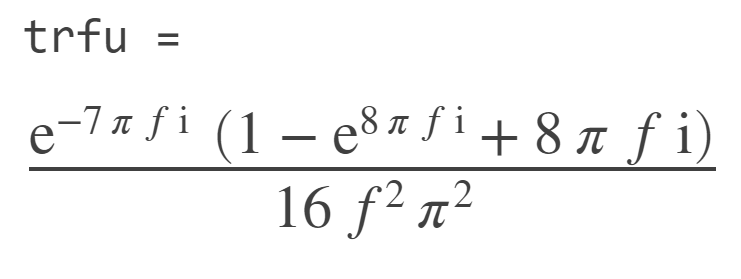
\includegraphics[width=0.5\linewidth]{img/ResultadoEcuacionMATLAB.png}
            \caption{Resultado de la simulación de la Transformada de Fourier de la señal.}
            \label{resultadoEcuacionMATLAB}
        \end{figure} 
        
        Realizando la comparación con la ecuación \ref{resultadoFT}, se evidencia que se trata de 
        la misma ecuación, por lo que se puede considerar que obtener la transformada de Fourier
        por medio de una integral simbólica es una buena alternativa. Además de comprobar el resultado
        numérico de los cálculos, se implementó en el algoritmo un ciclo capaz de evaluar el resultado
        de la figura \ref{resultadoEcuacionMATLAB} para poder representar las grafica del espectro de la
        frecuencia de la transformada de la señal planteada.
         
        \begin{figure}[H]
            \centering 
            \begin{subfigure}[h]{0.49\linewidth}
                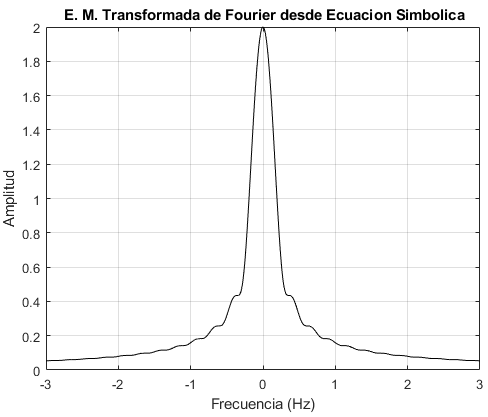
\includegraphics[width=\linewidth]{img/EMagnitudTF_ESimbolica.png}
                \caption{}
                \label{magnitudTeorica}
            \end{subfigure}
            \begin{subfigure}[h]{0.49\linewidth}
                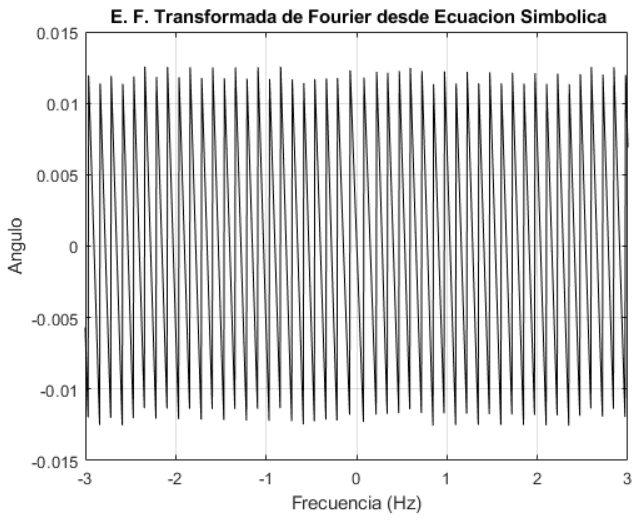
\includegraphics[width=\linewidth]{img/EFaseTF_ESimbolica.png}
                \caption{}
                \label{faseTorica}
            \end{subfigure}
            \caption{Gráficas del espectro de frecuencia de los cálculos simulados. (a) Espectro 
                    de magnitud, (b) Espectro de fase.}
            \label{espectroTeorico}
        \end{figure} 
        \vspace{-5mm}
    
        A partir de las figuras \ref{magnitudTeorica} y \ref{faseTorica} obtenidas en la simulación, se 
        realizaron comprobaciones con ayuda del algoritmo de la Transformada Rápida de Fourier (mencionada
        en la sección \ref{intro}). las gráficas obtenidas por el cálculo de la FFT se observan en la figura
        \ref{espectroFFT}.
        
        \begin{figure}[H]
            \centering 
            \begin{subfigure}[h]{0.49\linewidth}
                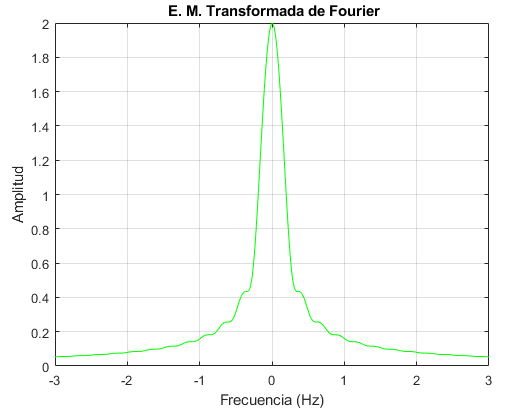
\includegraphics[width=\linewidth]{img/EMagnitudTF_FFT.png}
                \label{magnitudFFT}
                \caption{}
            \end{subfigure}
            \begin{subfigure}[h]{0.49\linewidth}
                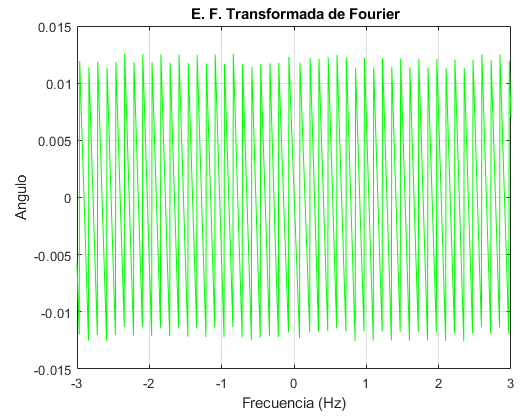
\includegraphics[width=\linewidth]{img/EFaseTF_FFT.png}
                \label{faseFFT}
                \caption{}
            \end{subfigure}
            \caption{Gráficas del espectro de frecuencia de FFT. (a) Espectro de magnitud, (b) Espectro de 
                    fase.}
            \label{espectroFFT}
        \end{figure}
        
        En la figuras \ref{magnitudFFT} y \ref{faseFFT} es evidente observar la similitud con las graficas en
        la figura \ref{espectroTeorico}, por lo que el método de evaluar una función obtenida a partir de una 
        integral simbólica, resulta ser efectiva para este tipo de actividades 
        
        espués de haber realizado estas validaciones para tener claridad acerca de lo que se 
        observa en las gráficas, se dio inicio a la investigación que se plantea en este documento
        con el análisis de algunos escenarios que se idearon en la simulación. las propiedades de 
        la Transformada de Fourier que se usaron para el análisis fueron:
        
        \begin{itemize}
            \item Multiplicación por un escalar.
            \item Cambio de escala.
            \item Traslación en el tiempo.
            \item Traslación en frecuencia.
        \end{itemize}
        
    \subsection{Desarrollo del objetivo clave 2--Cambio de amplitud en el dominio temporal - Linealidad}
        La propiedad de linealidad indica que al realizarse la transformada de una función multiplicada por un escalar, se obtendrá como resultado la misma transformada pero multiplicada por el escalar de la siguiente forma: 
        \begin{equation}
            A{x}(t) \rightarrow A\tilde{x}(f)
            \label{Linearidad}
        \end{equation}
        
        Para la verificación de esta propiedad se evaluaron dos escenarios, uno en el cual se realiza la transformada simbólica y la FFT sin ningún tipo de modificación a la señal original y otro escenario donde se multiplica la señal original por un escalar arbitrario:
        
        \begin{figure}[H]
            \centering 
            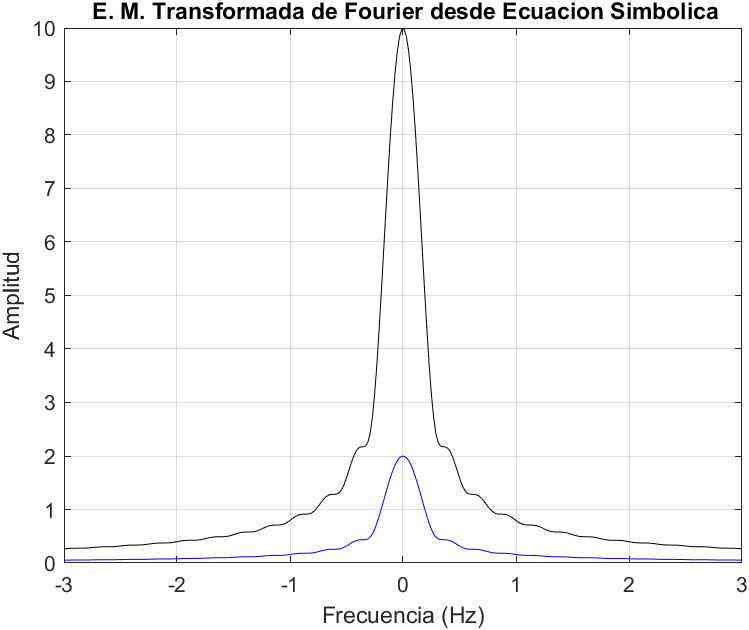
\includegraphics[width=0.5\linewidth]{img/Proplinearidad.png}
            \caption{Gráficas del espectro: (negro)  
                     Espectro de magnitud con amplitud 5, (azul) Espectro de magnitud original.}
             \label{P1}
        \end{figure}
        \vspace{-5mm}    
            
        Por inspección se confirma que la propiedad es aplicada correctamente al modificar los parámetros de la simulación para un escalar A=5. Por confirmación, se evalúa la transformada simbólica en dos puntos específicos de frecuencia 0 Hz y 1 Hz para obtener confirmación numérica de la aplicación de la propiedad y se obtienen los resultados esperados para la ecuación \ref{Linearidad}.
        
    \subsection{Desarrollo del objetivo clave 3--Cambio de escala}
        La propiedad de cambio de escala indica que al realizarse la transformada de una función con un cambio de proporción en su variable independiente, se obtendrá una transformada con relación inversamente proporcional a ese cambio de la siguiente forma: 
        
        \begin{equation}
            x(at)\rightarrow \frac{1}{\left | a \right |} \tilde X(\frac{f}{a})
            \label{Escala}
        \end{equation}
         
        Para la verificación de esta propiedad se evaluaron dos escenarios; uno en el cual se realiza la transformada simbólica y la FFT sin ningún tipo de modificación a la señal original y otro escenario donde se cambia la escala así:
        
            \begin{figure}[H]
                \centering 
                    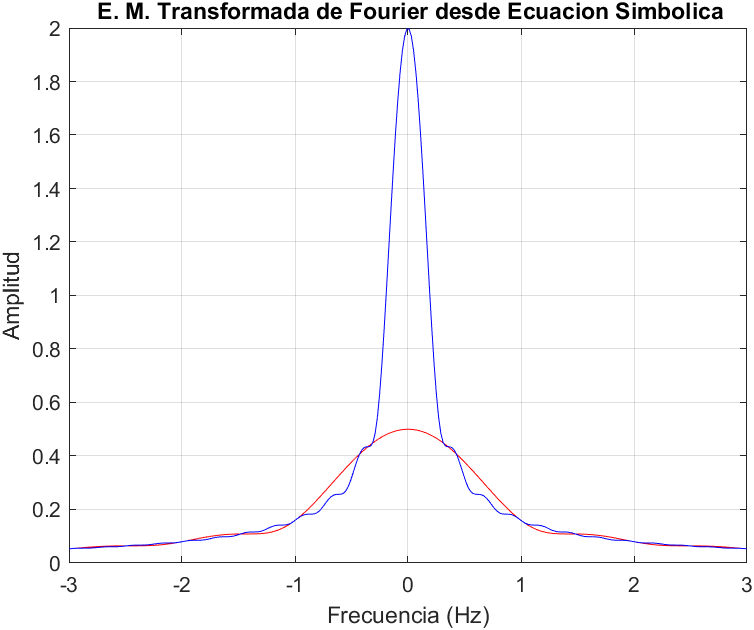
\includegraphics[width=0.5\linewidth]{img/Propescala.png}
                \caption{Gráficas del espectro: (rojo) Gráfica 
                        espectro de magnitud con escala esc=4, (azul) Gráfica espectro de magnitud original.}
                \label{P1}
            \end{figure}
            
        Se puede apreciar que al multiplicar la variable independiente "t" por un escalar esc=4, el espectro de magnitud tiene un comportamiento descrito por la notación (3). Este comportamiento tiene un efecto similar al que se encontró en el taller anterior cuando se modificó en periodo de la señal. Desde un punto de vista aritmético, cambiar la escala de una función periódica, equivale a cambiar escalarmente el periodo de su frecuencia fundamental.
        
    \subsection{Desarrollo del objetivo clave 4--Translación en el dominio temporal}
        La propiedad de translación en el tiempo indica que al realizarse la transformada de una función que tiene un desplazamiento temporal, se obtendrá como resultado la transformada de la función original pero multiplicada por un exponencial complejo de la siguiente forma: 
        
        \begin{equation}
            {x}(t-to) \rightarrow \tilde{X}(f) e^{-j2 \pi fto}
            \label{TTiempo}
        \end{equation}
        
        Para la evaluación de este escenario se hace necesario tener en cuenta la información entregada por el espectro de fase, ya que en la notación (4) es notorio que el resultado de aplicar un desplazamiento temporal únicamente va a tener efectos en la parte imaginaria de la transformada de Fourier debido a la forma del exponencial complejo que acompaña al par transformado.
        
        \begin{figure}[H]
                \centering 
                \begin{subfigure}[h]{0.49\linewidth}
                    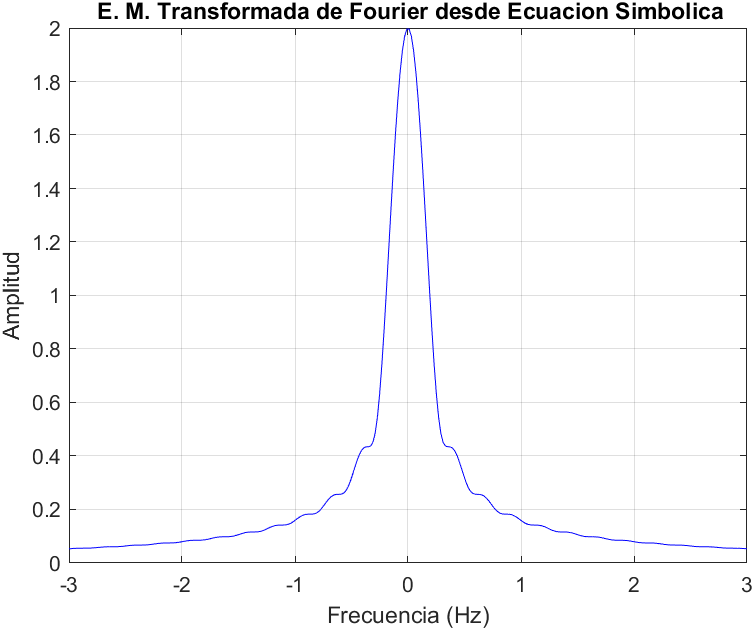
\includegraphics[width=\linewidth]{img/Proptiempomagnitud.png}
                    \label{P3}
                    \caption{}
                \end{subfigure}
                \begin{subfigure}[h]{0.49\linewidth}
                    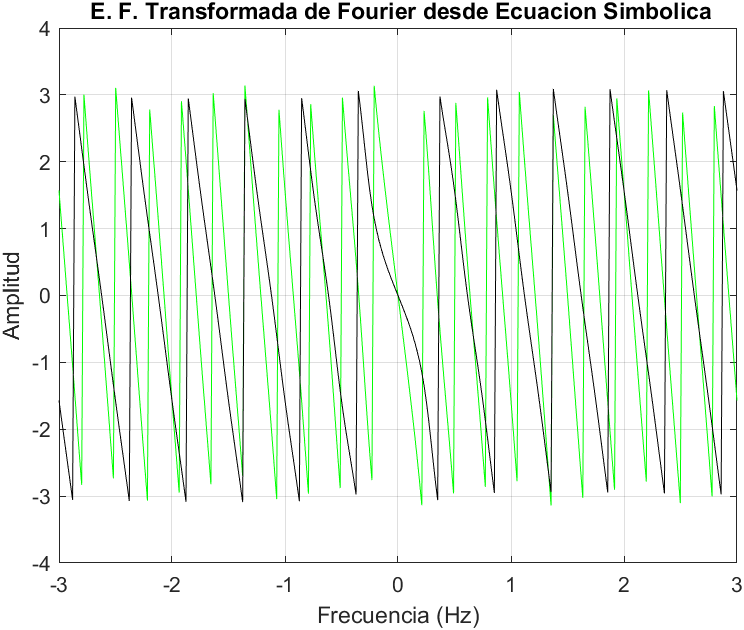
\includegraphics[width=\linewidth]{img/Proptiempofase.png}
                    \label{P33}
                    \caption{}
                \end{subfigure}
                \caption{(a) Superposición de espectros de magnitud, (b) Superposición de espectros de fase (verde) Fase sin aplicar desplazamiento - (negro) Fase al aplicar desplazamiento sh=2.}
                \label{P33}
            \end{figure}
        
        Al inspeccionar las gráficas obtenidas, se confirma que en el caso de translación temporal, el espectro de magnitud no sufre ninguna modificación; Sin embargo, el espectro de fase si cambia debido a que el movimiento de la señal en el dominio del tiempo refleja su información en la fase de la transformada.
        
    \subsection{Desarrollo del objetivo clave 5--Translación en el dominio de la frecuencia}
        La propiedad de translación en frecuencia indica que al realizarse la transformada de una función en el tiempo la cual esta multiplicada por un exponencial complejo tal que cause un cambio en la frecuencia, se obtendrá como resultado la misma transformada pero desplazada en el dominio de la frecuencia de la siguiente forma: 
        
        \begin{equation}
            {x}(t)e^{j2 \pi fot} \rightarrow \tilde{X}(f-fo)
            \label{TFrecuencia}
        \end{equation}
        
        Al realizar los cambios en la simulación, se obtuvieron los siguientes resultados:
        
        \begin{figure}[H]
                \centering 
                \begin{subfigure}[h]{0.49\linewidth}
                    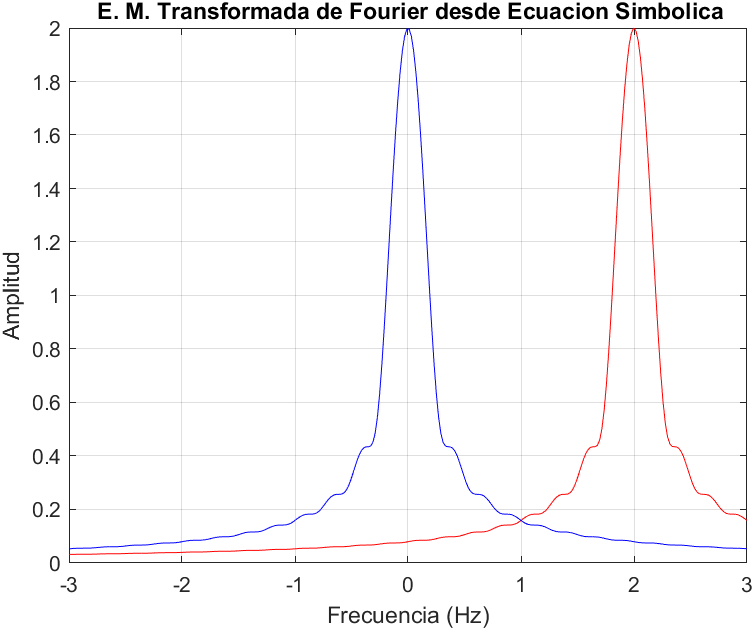
\includegraphics[width=\linewidth]{img/Propfrecmagnitud.png}
                    \label{P4}
                    \caption{}
                \end{subfigure}
                \begin{subfigure}[h]{0.49\linewidth}
                    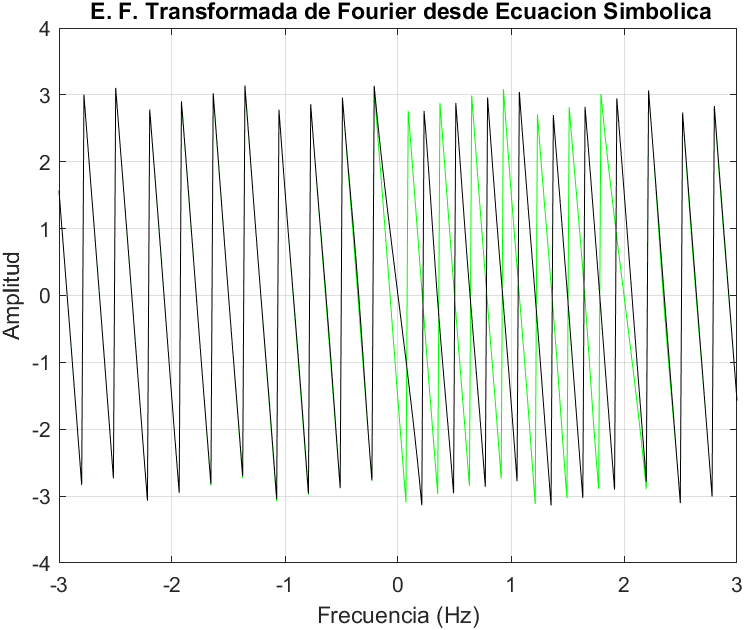
\includegraphics[width=\linewidth]{img/Propfrecfase.png}
                    \label{P44}
                    \caption{}
                \end{subfigure}
                \caption{(a) Superposición de espectros de magnitud, (b) Superposición de espectros de fase (verde) Fase sin aplicar desplazamiento - (negro) Fase al aplicar desplazamiento sh=2.}
                \label{P44}
            \end{figure}
            
\section{Conclusiones}
    En el dominio del tiempo cuando se tiene una señal de tiempo discreto o de periodo infinito,
    su magnitud en frecuencia tiende a ser cero en el infinito, por tanto sus valores de 
    intensidad decaen generando que su potencia promedio tienda a cero. Por ello se concluye 
    que al tratarse con señales de periodo infinito se define la energía total que existe en vez 
    de la potencia.
    
    Debido a una relación biunívoca que existe entre una función en el dominio del tiempo con su 
    dominio de frecuencia pueden formar únicamente un par transformado. por esta razón una señal 
    no puede tener dos o más transformadas de Fourier.
    
    La propiedad de cambio de escala muestra un efecto de compresión cuando su parámetro es 
    mayor a la unidad y de expansión cuando es menor a la unidad, así mismo su valor cuando es 
    negativo se produce su invertida, lo cual produce una modificación en el periodo. Por tanto
    los efectos de esta propiedad causara una modificación recíproca en la magnitud de la 
    frecuencia.
    
    
%\appendix
%\section{Cálculo teórico}

    %Realización de los cálculos matemáticos de la Transformada de Fourier de la señal 
    %asignada, la formula empleada para el cálculo de la transformada es la siguiente:

    %\begin{equation}
        %\tilde{x}(f)=\int_{-\infty}^{\infty}x(t)e^{-j2\pi ft} \mathrm{d}t
        %\label{transformadaFourier}
    %\end{equation}

    %Recordando que del primer trabajo, la función correspondiente a la pendiente de la 
    %gráfica se expresa de la siguiente manera:

    %\begin{equation}
        %x(t)=\frac{1}{4} t + \frac{1}{8}
        %\label{funcionLineal}
    %\end{equation}

    %Esta función lineal se encuentra limitada por un intervalo de duración $4$ segundos, como valor
    %mínimo se tiene $-\frac{1}{2}$ y valor máximo $\frac{7}{2}$, lo que hace que esta 
    %función se vea como un "diente de sierra", por tanto su función más representativa o
    %su intervalo descriptivo es el siguiente:
    
    %\begin{equation}
        %\begin{split}
            %x(t)&=\left(\frac{1}{4} t + \frac{1}{8}\right)rect\left(\frac{t}{4} + \frac{3}{8}\right) \\
                %&=  \left\lbrace  \begin{array}{ll}
                                    %\frac{1}{4} t + \frac{1}{8}; & -\frac{1}{2} \leq t \leq \frac{7}{2} \\
                                    %0; & p.o.c.
                                %\end{array}
                    %\right.      
        %\end{split}
        %\label{dienteSierra}
    %\end{equation}

    %El proceso para obtener la Transformada de Fourier de la ecuación \ref{dienteSierra} 
    %se realiza a continuación, donde el valor $x(t)$ de la ecuación \ref{transformadaFourier} será la 
    %ecuación \ref{funcionLineal}, y el valor de los intervalos de la integral serán los que 
    %limitan la función lineal, como se menciono anteriormente \cite{silviaRB}: 

    %\begin{equation*}
        %\begin{split}
            %\tilde{x}(f)& = \int_{\frac{3}{2} -2}^{\frac{3}{2} +2}\left(\frac{1}{4} t+\frac{1}{8} \right) e^{-j2\pi ft}\mathrm{d}t \\
                        %& = \frac{1}{4} \int_{\frac{3}{2}-2}^{\frac{3}{2}+2}t e^{-j2\pi ft}\mathrm{d}t + \frac{1}{8} \int_{\frac{3}{2} -2}^{\frac{2}{3} +2} e^{-j2\pi ft}\mathrm{d}t \\
                        %& = e^{-j2\pi ft}\left(\frac{jt}{8\pi f}  + \frac{1}{16\pi ^{2} f^2}  + \frac{j}{16\pi f} \right)  \Big|_{\frac{3}{2} -2}^{\frac{3}{2} +2} \\
                        %& = \frac{je^{-j3\pi ft } e^{-j4\pi ft}}{8\pi f} \left[\frac{1}{j2\pi f} + 4 
                          %- e^{j8\pi ft} \left(\frac{1}{j2\pi f} \right)\right] \\
                        %& = \left[\left(\frac{1}{16\pi^2 f^2}+\frac{j}{2\pi f}\right)e^{-j4\pi f}-\frac{e^{j4\pi f}}{16\pi^2 f^2}\right] e^{-j3\pi f} \\
        %\end{split}
    %\end{equation*}  
  

    %\begin{equation}
        %\tcboxmath[colback=gray!25!white,colframe=black, title=Transformada de Fourier]{
            %\tilde{x}(f) = \frac{e^{-j7pi f }(1 - e^{j8\pi f} + j8\pi f)}{16\pi^2 f^2}
        %}
    %\end{equation}

\printbibliography[title={Bibliografía}]

\end{document}
